\textit{This chapter was adapted from an interactive blog post on}
\href{https://learningmechanics.pub/deep-linear-nets/}{learningmechanics.pub}
\textit{co-authored by Dhruva Karkada, Jamie Simon, and yours truly.}

\bigskip

In the previous chapter, we argued that the difficulty of studying deep neural networks comes down to three axes of complexity: coupled dynamics, pointwise nonlinearities, and data complexity. We also learned about the learning mechanic's go-to approach to tackling these axes: turning one off, and seeing how far the resulting \textit{toy model} can carry us.

In this chapter we turn off the second axis. We keep depth, we keep coupled dynamics, and we maintain a mostly data-agnostic approach, but we throw away the nonlinearities. What remains is a \emph{deep linear network}: a deep neural network with no nonlinear activation functions:

\begin{align*}
    \hat{f}(x) = W_L \cdots W_2 W_1 x.
\end{align*}

In Chapter 1, we solved the training dynamics of the simplest linear model: linear regression (Equation~\eqref{linreg}). Doing so revealed that 1) the loss decays exponentially, and 2) out of the infinitely many interpolating solutions, gradient descent picks the one with smallest L2 norm. Those were amusing results, but they didn't teach us much about the deep neural networks we're actually interested in because we had thrown away too much complexity. By dropping to a single layer, we killed off the coupled dynamics in addition to the nonlinearities, and coupled dynamics are exactly where a lot of the interesting behavior lives.

This time we keep the coupling. We do so by holding on to depth ($L > 1$), which means several weight matrices influence each other's gradients, and we ask what that coupling alone---with no nonlinearity---can produce. The answer, remarkably, is \emph{a lot}. The following are four pieces of folklore about how real neural networks train. They're the kind of empirical findings that the research community might observe and be interested in, but often lack a precise account of \textit{why}:
\begin{enumerate}
    \item networks preferentially learn certain functional directions before
    others;\footnote{This is a kind of inductive bias, much like the
    minimum-norm bias of gradient descent in linear regression from the previous
    chapter.}
    \item networks reliably find good (and sometimes globally optimal) minima,
    despite living in a wildly nonconvex loss landscape;
    \item at any given moment in training, each weight matrix's update is
    approximately low-rank compared to the matrix itself; and
    \item networks sometimes learn in a stepwise fashion---long flat plateaus
    interrupted by sudden drops in the loss---especially when trained from very
    small initial weights.
\end{enumerate}

The claim of this chapter is that deep linear networks reproduce \emph{all four} of these behaviors, in a single system we can solve with pen and paper.

\section{Setting up the problem}

Before we can solve anything, we need to write down the setting precisely. Suppose we have a dataset $\Dcal = \{ (x_i, y_i) \}_{i=1}^n$ of $n$ sample-target pairs, where both the samples $x \in \R^{d_\text{in}}$ and the targets $y \in \R^{d_\text{out}}$ are vectors. Our deep linear network passes an input through a chain of matrix multiplications,

\begin{equation}
    \hat{f}(x) = W_L \cdots W_2 W_1 x,
\end{equation}

where the weight matrices $\{ W_\ell\}_{\ell=1}^L$ are learned through training so that $\hat{f}(x_i) \approx y_i$. The network is \emph{deep} because it has $L > 1$ trainable layers stacked on top of one another. And it's \emph{linear} because, no matter how many matrices we multiply together, the result is still a single linear map: we can collapse the whole chain into $\hat{f}(x) = W_\text{tot}\, x$, where $W_\text{tot} := W_L \cdots W_1$. So as a \emph{function}, this thing is no more expressive than ordinary linear regression. Of course, the interesting part isn't the function it can represent---it's the \emph{path gradient descent takes to get
there}, and that path turns out to be genuinely nonlinear.

As usual, we train by minimizing the mean squared error with gradient descent:
\begin{align*}
    \Lcal(W_1, \dots, W_L)
    = \frac{1}{n} \sum_{i=1}^{n} \|y_i - W_L \cdots W_1 x_i\|^2.
\end{align*}

Now we'll do a small piece of bookkeeping that pays off enormously later: we'll rewrite this loss so that the data only shows up through a couple of summary matrices, rather than through every individual example. The sum over examples is
really an average over the dataset, so we can write the loss as an expectation
and do some matrix algebra to simplify the expression:\footnote{Filling in the ``some matrix algebra''
step---expand the trace and complete the square---is left as an exercise at the
end of the chapter.}
\begin{align}
    \Lcal(W_1, \dots, W_L)
    &= \mathbb{E}_{(x,y)\sim\Dcal}
       \Big[\Tr\, (y - W_L \cdots W_1 x)(y - W_L \cdots W_1 x)^\top \Big] \notag \\
    &= \|\Sigma_{yx}\Sigma_{xx}^{-1/2} - W_L \cdots W_1 \Sigma_{xx}^{1/2}\|_\mathrm{F}^2
       + \mathrm{const.} \label{eq:matrix-loss}  
\end{align}

Two new objects appeared here, and they're the only way the data will ever enter
our analysis, so let's name them carefully. The first,
$\Sigma_{xx} := \mathbb{E}_\Dcal[xx^\top]$, is the \textbf{input-input
covariance}---it records how the input features vary together, with no reference
to the targets at all. The second, $\Sigma_{yx} := \mathbb{E}_\Dcal[yx^\top]$, is
the \textbf{output-input covariance} (sometimes the input-output correlation)---it
records how inputs and targets co-vary, and so it's where the actual input-to-output relationship we're trying to learn is stored. All of the statistical structure in the data that the network can possibly learn from is packed into these two matrices. Everything downstream depends on the data only through $\Sigma_{xx}$ and $\Sigma_{yx}$.

A note on Equation~\eqref{eq:matrix-loss}: the $\|\cdot\|_\mathrm{F}$ here is the \emph{Frobenius norm}, which just sums the
squares of all of a matrix's entries---the matrix version of the ordinary vector
length. And the constant term, written out in the footnote,\footnote{$\mathrm{const.}
= \Sigma_{yy} - \Sigma_{yx}(\Sigma_{xx})^{-1}(\Sigma_{yx})^\top$, which is constant
with respect to the weight matrices.} doesn't depend on the weights at all. You
can think of it as irreducible noise---a floor on the loss that's there no matter
what we do with the weights, so we're free to ignore it when we differentiate.

\section{Solving the learning dynamics}

Like in the linear regression example in Chapter 1, we'll attempt to exactly solve for the learning dynamics of a deep linear network; i.e., write down a formula for what the weights look like at any moment during training. We'll follow a streamlined version of the classic derivation from
\href{https://arxiv.org/pdf/1312.6120}{Saxe et al.\ (2013)}. And to keep the algebra easier to follow, we'll only do the $L = 2$ case in full. (The strategy for deeper networks is essentially identical, just more tedious.)

Here's a bird's-eye view of the plan we will execute:

\begin{enumerate}
    \item \textbf{Write the equations of motion.} We'll write down the gradient
    descent updates, take the infinitesimal-learning-rate limit (gradient flow)
    from last chapter, and end up with differential equations for how the weight
    matrices evolve in time.
    \item \textbf{Make the equations tractable.} We'll look at those equations,
    decide they're too hard as written, and add one assumption---that the input
    data is ``whitened,'' meaning $\Sigma_{xx} = I$.
    \item \textbf{The hard part: alignment.} We'll argue that when the weights
    start out very small, the early phase of training mostly does one thing: it
    rapidly rotates the weight matrices into alignment with each other and with
    the target, before their magnitudes have grown much.
    \item \textbf{Decouple and solve.} Once aligned, the matrix dynamics fall
    apart into independent one-dimensional problems. We integrate those, and out
    pops a clean sigmoidal learning curve for each ``direction'' in the data.
\end{enumerate}

\subsection{Step 1: Write the gradient flow equations}

Our first job is to get from ``minimize this loss with gradient descent'' to an actual set of differential equations we can try to solve. For a 2-layer network, the loss is
\begin{align*}
    \Lcal(W_1, W_2) = \frac{1}{n} \sum_{i=1}^{n} \|y_i - W_2 W_1 x_i\|^2.
\end{align*}
To keep the bookkeeping as light as possible, we'll assume everything is square:
inputs $x_i \in \R^d$, targets $y_i \in \R^d$, and $d$ hidden neurons in between,
so that $W_1$ and $W_2$ are both $d \times d$ (none of the conclusions actually
need this; the general rectangular case works the same way with more indices to
track).

Plain gradient descent with learning rate $\eta$ updates the weights in discrete
steps:
\begin{align*}
    W_1^{(t+1)} &= W_1^{(t)} - \eta \nabla_{W_1}{\Lcal}\big|_{W_1^{(t)}} \\
    W_2^{(t+1)} &= W_2^{(t)} - \eta \nabla_{W_2}{\Lcal}\big|_{W_2^{(t)}}.
\end{align*}

Analyzing discrete steps is pretty much intractable. So we'll turn to a tool introduced in the previous chapter: gradient flow, i.e., infinitesimally small learning rate. This replaces the jumpy update rule with a smooth differential equation in continuous time:
\begin{align*}
    \frac{d}{dt}W_\ell = -\nabla_{W_\ell}{\Lcal}.
\end{align*}

Now we just need the gradients. Computing them in terms of the two covariance
matrices we defined above gives our \textbf{equations of motion} for the network:
\begin{align}
    \frac{d}{dt}W_1 &= W_2^\top(\Sigma_{yx} - W_2 W_1 \Sigma_{xx})\label{eq:W1}\\
    \frac{d}{dt}W_2 &= (\Sigma_{yx} - W_2 W_1 \Sigma_{xx}) W_1^\top .\label{eq:W2}
\end{align}

Before we try to solve these, let's just read them and get a feel for what they're saying---this kind of ``what is this equation telling me physically'' pause is always worth taking.

Look at the parenthesized term, $\Sigma_{yx} - W_2 W_1 \Sigma_{xx}$. This is the engine driving both updates; essentially a \textit{residual} term, i.e., the gap between the actual structure in the data ($\Sigma_{yx}$) and the structure the model has currently learned ($W_2 W_1 \Sigma_{xx}$). Assuming small initialization, early in training, when the weights are still tiny, the product $W_2 W_1 \Sigma_{xx}$ is negligible compared to $\Sigma_{yx}$, so the whole update is dominated by $\Sigma_{yx}$---the input-output relationship. In other words, \emph{early learning is steered by the data's input-output structure}, with the
input covariance $\Sigma_{xx}$ playing only a supporting role, gently reshaping the gradient\footnote{This is kind of matrix that rescales the gradient before it's applied is called a \textit{preconditioner}.}. And what about the end of training? Training stops when the weights stop moving, i.e., when $\frac{d}{dt}W_1 = \frac{d}{dt}W_2 = 0$. Reading off the equations,
that happens when $W_2 W_1 = \Sigma_{yx}\Sigma_{xx}^{-1}$.

There's another interesting observation we can make from these equations. Notice how similar they look. If you right-multiply the first by $W_1^\top$ and left-multiply the second by $W_2^\top$, you find that both equal the same thing:
\begin{align*}
    \Big(\tfrac{d}{dt}W_1\Big)W_1^\top = W_2^\top\Big(\tfrac{d}{dt}W_2\Big).
\end{align*}
Rearranging, this says that a particular combination of the weights never changes
during training:
\begin{equation}
    \frac{d}{dt}\big(W_2^\top W_2 - W_1 W_1^\top\big) = 0.
    \label{eq:conservation}
\end{equation}

A quantity that stays fixed while everything around it evolves is called a
\textbf{conservation law}---the same idea as conservation of energy or momentum in
physics, where some combination of the moving parts stays pinned no matter how
violently the system thrashes around. Here the conserved quantity is the matrix
\begin{align*}
    H := W_2^\top W_2 - W_1 W_1^\top,
\end{align*}
which measures the imbalance between the two layers. When $H \approx 0$, the two
layers sit in a kind of equilibrium with each other, and we say the weights are
\textbf{balanced}.

The algebraic derivation of the conservation law above actually obscures a deeper mechanism. The function that a deep linear network defines has a \emph{continuous symmetry}: it doesn't change if we shrink one layer while correspondingly stretching the next, $W_2W_1 = (W_2A^{-1})(AW_1)$ for any invertible matrix $A$. This symmetry is baked into the fact that we built our model by multiplying matrices together. And it's is the "true" source of the conservation law. Physicists will recognize the symmetry-implies-conservation pattern from Noether's theorem. While Noether's theorem doesn't directly apply here, the symmetry really does produce the conserved quantity directly\footnote{See exercise at the end of the chapter.}. The conservation law is, at its root, the architecture's symmetry made visible in the dynamics.

An interesting insight we can gain from the conservation law is that the geometry of optimization is highly constrained. Because $H$ can never change, the trajectory the weights trace out is confined to a surface of constant $H$, which turns out to be hyperbolic in character.\footnote{For intuition, the scalar version $\frac{d}{dt}(x^2 - y^2) = 0$ says $x^2 - y^2$ is constant; which is exactly the
equation of a hyperbola.} Note that a similar conservation law holds for arbitrarily deep linear networks. Thus, hyperbolic trajectories are a fundamental phenomenon of optimizing linear models using gradient descent.

The conservation law, like any conservation law in physics, allows us to reduce the degrees of freedom in the system. Concretely, the fact that $H$ is pinned for all time means that if we initialize the weights small (so $H$ starts tiny), we get to \emph{assume} the layers stay
balanced throughout training (i.e., $H$ stays tiny). This fact will become useful later. 

\subsection{Step 2: Whiten the input data}

We now have our equations of motion, but integrating them at this point doesn't seem promising. The trouble is that the matrices $\Sigma_{yx}$ and $\Sigma_{xx}$ are tangled together inside the dynamics. These two matrices generally won't \emph{commute}. Since each matrix has its own natural set of axes (its singular
vectors), we end up with two conflicting sets of natural axes.\footnote{Two diagonalizable matrices (for instance, symmetric ones) commute if and only if they share a common eigenbasis---that is,
the same set of natural axes.} The dynamics are being pulled toward two misaligned
coordinate systems at once, and that tension is exactly what makes the equations
so hard to integrate.

The most straightforward resolution is to force commutativity. We achieve this by \emph{whitening} the input data: we apply a fixed linear
transformation to the inputs that makes their covariance equal to the identity,
$\Sigma_{xx} = I$. Whitening just means ``decorrelate and rescale the input
features so they have unit variance and no cross-correlations''---and crucially,
you can always do this as a preprocessing step before training ever
begins.\footnote{This is a perfectly legitimate thing to do to your data, so it's
not a crazy assumption. Whether it faithfully reflects what happens in real ML
pipelines, where people don't usually whiten, is a separate and fair question.} Our equations of motion then collapse to
\begin{align}
    \frac{d}{dt}W_1 &= W_2^\top(\Sigma_{yx} - W_2 W_1) \label{eq:W1-whitened}\\
    \frac{d}{dt}W_2 &= (\Sigma_{yx} - W_2 W_1) W_1^\top\label{eq:W2-whitened}.
\end{align}
Much cleaner. Now only one data matrix remains in the equations: $\Sigma_{yx}$.

\subsubsection*{Finding the right basis}

A great deal of applied math and physics comes down to a single move: \emph{find
the coordinate system in which your problem becomes simple.} The whole point of whitening was to isolate such a coordinate system. After whitening, all the data-dependent structure in our equations lives in the single matrix $\Sigma_{yx}$. The right tool to extract a natural set of axes from it is the \textbf{singular value decomposition (SVD)}, which factors any matrix into a
rotation, a set of nonnegative stretch factors, and another rotation:
\begin{align*}
    \Sigma_{yx} := U^\star \Lambda^\star {V^\star}^\top.
\end{align*}
Here $V^\star$ holds the input-side axes, $U^\star$ holds the output-side axes,
and $\Lambda^\star$ is diagonal, holding the stretch factors---the \emph{singular
values}---that say how strongly each input axis maps to its partner output axis.

Now we rotate our whole problem into this frame. We define new ``tilde'' versions
of the weights, measured in $\Sigma_{yx}$'s coordinate system:
\begin{align*}
    \Lambda^\star := {U^\star}^\top \Sigma_{yx} V^\star, \qquad
    \tilde{W}_1 := W_1 V^\star, \qquad
    \tilde{W}_2 := {U^\star}^\top W_2.
\end{align*}
Substituting these in, the equations of motion keep their exact shape but with
$\Sigma_{yx}$ replaced by the diagonal $\Lambda^\star$:
\begin{align}
    \frac{d}{dt}\tilde{W}_1 &= \tilde{W}_2^\top(\Lambda^\star - \tilde{W}_2 \tilde{W}_1)
    \label{eq:W1-diag}\\
    \frac{d}{dt}\tilde{W}_2 &= (\Lambda^\star - \tilde{W}_2 \tilde{W}_1) \tilde{W}_1^\top
    \label{eq:W2-diag}.
\end{align}

Since we initialize the weights randomly and isotropically---with no
preferred direction of their own---rotating the coordinate axes leaves the
\emph{distribution} of initial weights statistically unchanged. The rotated
problem is therefore exactly equivalent to the original one. We've paid nothing
and gained a target matrix $\Lambda^\star$ that is now diagonal, with real,
nonnegative singular values $\lambda^\star_\mu$ (nonnegative because $\Sigma_{yx}$
is positive-semidefinite).

By rotating into the SVD basis of $\Sigma_{yx}$,
we've revealed that the data is not one tangled blob but a stack of independent,
orthogonal pieces, which we'll call \textbf{modes}. Each mode $\mu$ couples one
\emph{input direction} (the $\mu$-th column of $V^\star$) to one \emph{output
direction} (the $\mu$-th column of $U^\star$), and the singular value
$\lambda^\star_\mu$ tells you how prominent that particular input-output
association is in the data. As a rule of thumb, large singular values correspond
to coarse, dominant structure, and small singular values to fine details---a fact
that will become the whole story when we get to the order in which things are
learned.

\subsubsection*{An enlightening example about the SVD}

This mode business can feel abstract, so let's ground it in a concrete example,
due to \href{https://www.pnas.org/doi/10.1073/pnas.1820226116}{Saxe et al.\
(2019)}. This is also a nice chance to do what we always try to do in this
course---check that our abstractions correspond to something real and
interpretable.

Imagine the network is shown an item $i$---say, a ``Canary''---encoded as a
one-hot input vector $x_i$ (a vector that's all zeros except for a single $1$
picking out ``Canary''). Its job is to predict a vector of features $y_i$: ``Can
Fly,'' ``Has Wings,'' ``Is Yellow,'' and so on. Over training it sees many such
item-feature pairs, and the statistical structure of this little world is
summarized, as always, by the output-input correlation matrix
$\Sigma_{yx} = \mathbb{E}_{\Dcal}[y_i x_i^\top]$.

\begin{figure}[H]
    \centering
    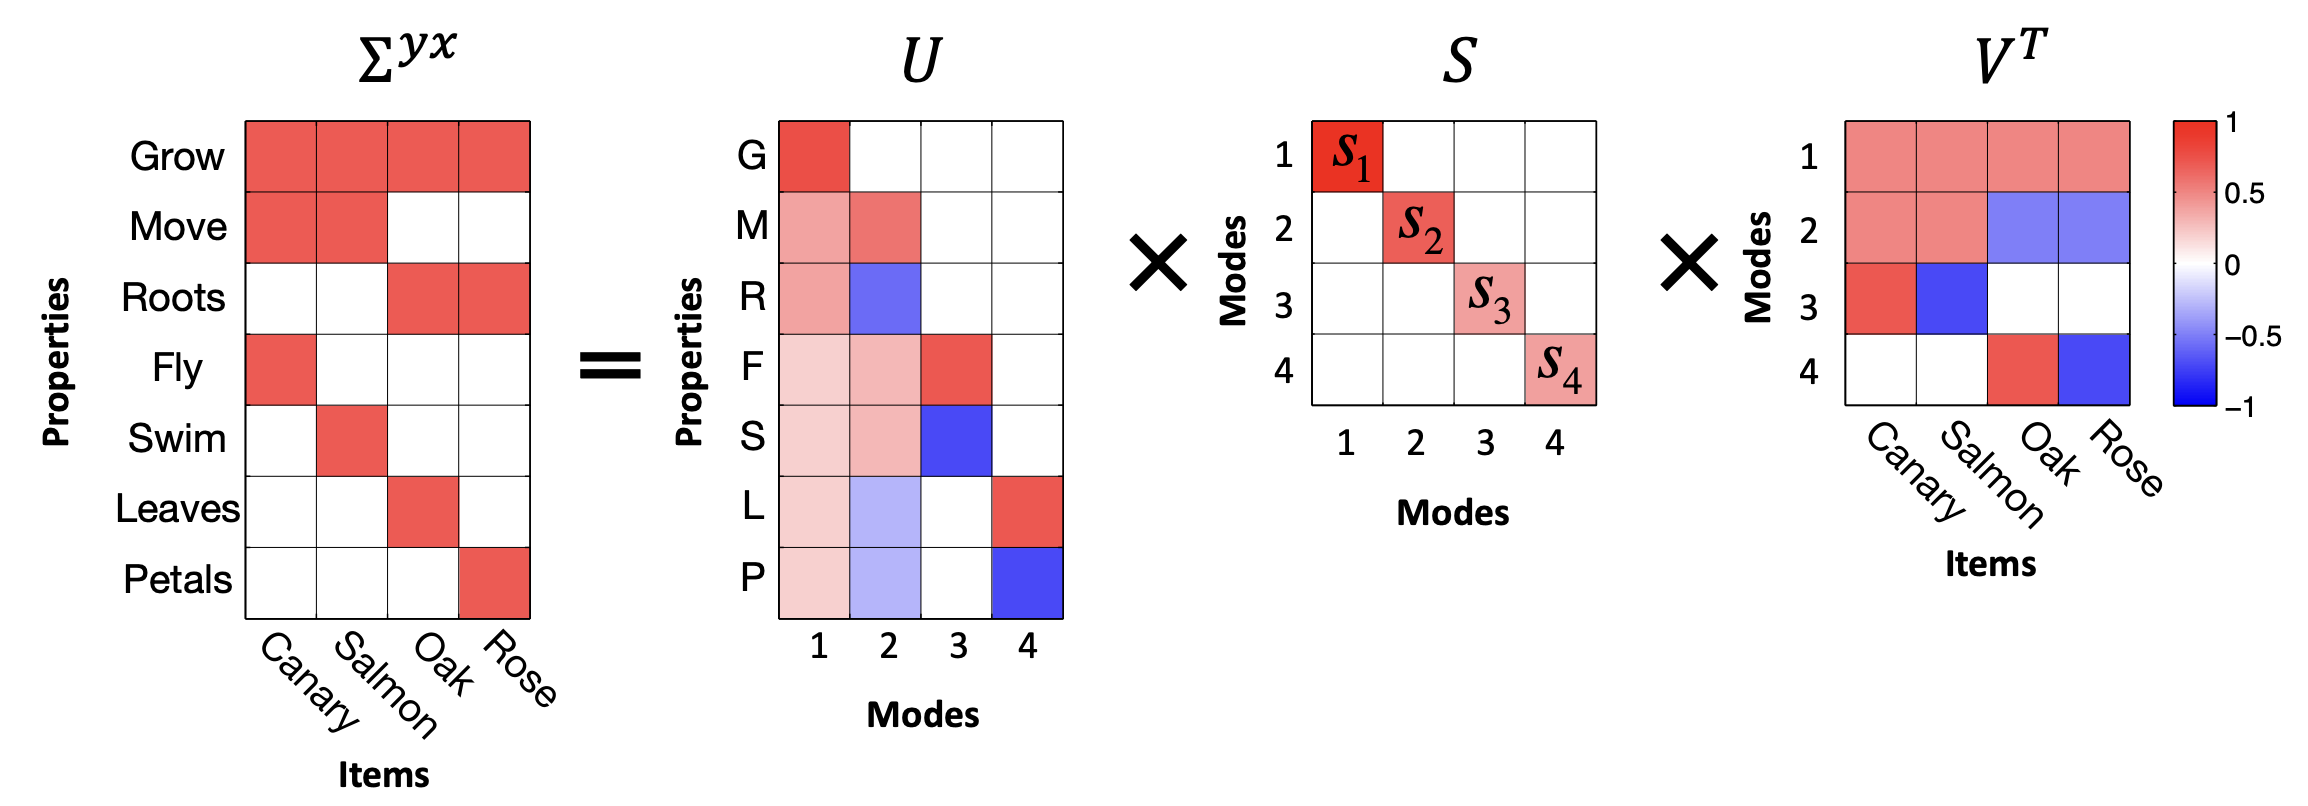
\includegraphics[width=0.8\linewidth]{figures/ch2-svd.png}
    \caption{Modes link a set of coherently covarying properties with a set of
    coherently covarying items.}
    \label{fig:ch2-svd}
\end{figure}

Now we can give the SVD's two sets of axes a tangible meaning.

The columns of $V^\star$ (equivalently, the rows of ${V^\star}^\top$) are the
\textbf{input modes}, or input-analyzing vectors. Each one places every input
item along a single interpretable semantic axis. The second input mode, for
instance, behaves like an ``animal--plant'' axis: animals like Canary and Salmon
land on the positive side, plants like Oak and Rose on the negative side. A single
direction in the input space has captured a coherent semantic distinction.

The columns of $U^\star$ are the \textbf{output modes}, or output-analyzing
vectors. Symmetrically, each one places every output \emph{feature} along a
semantic axis. Every input mode is paired with exactly one output mode, and the
singular value $\lambda^\star_\mu$ joining them measures that axis's
``categorizing power''---how much of the data's structure this one input-output
distinction accounts for. Big singular values are the broad, important cuts
through the data (animal vs.\ plant); small ones are the subtle, subordinate
details (which specific kind of bird).

The thing to take away---and the reason this example is worth dwelling on---is that
the SVD isn't just an algebraic convenience we reached for to make an integral
tractable. It is carving the data up along genuinely meaningful semantic
directions, and those very directions, as we're about to see, are the directions
the network learns \emph{one at a time, in order of importance}.

\subsection{Step 3: Argue that weight alignment happens quickly}

Our diagonalized equations of motion are cleaner than before, but they're still
coupled: $\tilde{W}_1$ and $\tilde{W}_2$ both appear inside each other's updates,
so we can't yet solve for either one on its own. The entire goal of this step is
to find a condition under which the coupling falls apart---under which the
dynamics \emph{decouple} into a bunch of independent one-dimensional problems we
can integrate by hand.

We're going to proceed by identifying a special condition (we'll call it \emph{weight alignment}) that, if true, makes everything decouple. Then we're going to argue---somewhat informally---that small initialization makes
this condition come true very quickly, early in training. We will \emph{not} prove
this rigorously. Instead we'll do something that is, in its own way, just as convincing, and we'll come back to it at the end of the next step.

\subsubsection*{What condition would decouple the dynamics?}

To find the condition we want, it helps to keep thinking spectrally---that is, in
terms of the SVD. Recall that the SVD splits any matrix into \emph{directions}
(the singular vectors, $U$ and $V$) and \emph{magnitudes} (the singular values,
$S$). The coupling in our equations lives entirely in the \emph{directions}. If the directional parts of the two weight matrices were
already settled and pointing the right way, the only thing left to evolve would be
the magnitudes---and magnitudes are just numbers, which decouple easily.

So let's write each weight matrix in its SVD form, $W_1 = U_1 S_1 V_1^\top$ and
$W_2 = U_2 S_2 V_2^\top$, and ask: under what directional conditions does the
model $\tilde{W}_2 \tilde{W}_1$ collapse to a clean product of magnitudes,
$S_2 S_1$, with all the rotation matrices canceling out? Working it
through,\footnote{To see it, write the rotated model in terms of the weight SVDs:
$\tilde{W}_2 \tilde{W}_1 = (U^{\star\top} W_2)(W_1 V^\star) = U^{\star\top}U_2\,
S_2\, V_2^\top U_1\, S_1\, V_1^\top V^\star$. Now impose the three conditions:
$U_2 = U^\star$ makes $U^{\star\top}U_2 = I$; $V_2 = U_1$ makes $V_2^\top U_1 = I$;
and $V_1 = V^\star$ makes $V_1^\top V^\star = I$. All the rotation matrices
collapse to identities and we're left with $\tilde{W}_2 \tilde{W}_1 = S_2 S_1$, a
product of pure magnitudes.} you need three things to line up:
\begin{enumerate}
    \item $U_2 = U^\star$ --- the output directions of $W_2$ match the data's
    output modes.
    \item $V_1 = V^\star$ --- the input directions of $W_1$ match the data's input
    modes.
    \item $V_2 = U_1$ --- the directions where $W_1$ ``hands off'' to $W_2$ match
    each other.
\end{enumerate}

We'll call these three conditions together \textbf{weight alignment}. Conditions 1
and 2 say the network is aligned with the \emph{data} (its ends point along the
data's modes); condition 3 says the two layers are aligned with \emph{each other}
(they interface cleanly, with no rotational mismatch in the middle). When all
three hold, only the singular values along the diagonals of $S_1$ and $S_2$ are left to evolve, and---as we'll confirm in Step 4---those evolve independently, mode by mode. That's the
decoupling we're after.

\subsubsection*{Why small initialization gets us there}

These three conditions are demanding, and there's no reason a randomly initialized
network should satisfy them. So why should we expect alignment to happen at all?

The answer is that it reliably happens, fast, in one specific setting: the
\textbf{small initialization regime}, where we start all the weights very close to
zero so that they have to \emph{grow} substantially over training. This is in
contrast to the \emph{large initialization} or ``lazy'' regime, where weights
start big and barely move from their random starting point---in which case no
interesting directional structure ever develops, and none of the phenomena in
this chapter appear. We'll have more to say about that contrast later. Small
initialization forces alignment through two separate mechanisms, one for the
layers-with-each-other condition and one for the layers-with-data conditions.

We'll sketch both. Feel free to skim these---the precise arguments lean on a bit
of perturbation theory and on power iteration, and the original
\href{https://arxiv.org/pdf/1312.6120}{Saxe et al.\ (2013)} derivation simply
\emph{assumed} fast alignment without proving it. The takeaway you actually need
is just that \emph{from small initialization, alignment happens quickly.}

\paragraph{Inner alignment (the layers align with each other), via the
conservation law.} Here we get to spend the conservation law we banked in Step 1.
Recall $H := W_2^\top W_2 - W_1 W_1^\top$ is conserved for all time. From small
initialization, the weights start tiny, so $H$ starts tiny---and because it's
conserved, it \emph{stays} tiny even after the weights have grown large. That
means that once training is underway,
\begin{align*}
    W_2(t)^\top W_2(t) = W_1(t) W_1(t)^\top + \text{(a tiny perturbation)}.
\end{align*}
This near-equality of the two layers' Gram matrices is what we earlier named
\textbf{balancedness} ($H \approx 0$). And balancedness is enough to pin the
layers' directions together, by way of a classical result called the
\textbf{Davis--Kahan $\sin\theta$ theorem}. In plain terms, that theorem says: if
two symmetric matrices differ only by a small amount, \emph{and} their own
eigenvalues are well separated from each other, then they must share essentially
the same eigenvectors. Here the two matrices are $W_1 W_1^\top$ and $W_2^\top W_2$,
they differ only by the tiny $H$, and small initialization makes their eigenvalue
gaps grow large compared to $\|H\|$---so the theorem applies and forces their
relevant directions to coincide. That's precisely condition 3, inner alignment
($V_2 = U_1$). (A companion fact, Weyl's inequality, similarly forces the two
layers' singular \emph{values} to agree---which we'll use in Step 4.)

\paragraph{Outer alignment (the layers align with the data), via power iteration.}
The conservation law explains why the two layers snap to each other, but not why
they snap to the \emph{data's} modes. For that, look again at the whitened
equation of motion at the very start of training:
\begin{align*}
    \frac{d}{dt}W_1 = W_2^\top(\Sigma_{yx} - W_2 W_1).
\end{align*}
At initialization the weights are minuscule, so $W_2 W_1 \ll \Sigma_{yx}$ and that
term is negligible. The update simplifies to
\begin{align*}
    \frac{d}{dt}W_1 \approx W_2^\top \Sigma_{yx}.
\end{align*}
Look at what this is doing: at each instant the weights are getting multiplied by
$\Sigma_{yx}$ again and again. Repeatedly multiplying a vector (or matrix) by a
fixed matrix is exactly \textbf{power iteration}, the standard algorithm for
extracting a matrix's \emph{dominant} direction---because the largest singular
value gets amplified the most with each multiplication, it quickly drowns out the
rest. So this early phase acts like power iteration on $\Sigma_{yx}$: it
aggressively rotates $W_1$'s top directions to point along $\Sigma_{yx}$'s top
directions ($V_1 \to V^\star$), which is conditions 1 and 2, outer alignment. By
the time the weights have grown enough that the $W_2 W_1$ term stops being
negligible, this rotation is already a done deal---the directions are locked, and
only magnitudes remain to evolve.

So both mechanisms point the same way: from small initialization, the network
rushes into alignment before it does much else. We'll \emph{assume} alignment
holds from here on. We'll empirically justify this assumption later on as well.

\subsection{Step 4: Decouple the dynamics and solve}

Now let's use the alignment assumption to actually solve for the learning curve.
The plan: impose alignment to kill the directional coupling, reduce the matrix
equations to a single scalar ODE per mode, and integrate that ODE in closed form.

With alignment assumed, our equations of motion involve only the (diagonal)
singular-value matrices:
\begin{align}
    \frac{d}{dt}S_1 &= S_2 (\Lambda^\star - S_2 S_1)\\
    \frac{d}{dt}S_2 &= (\Lambda^\star - S_2 S_1) S_1.
\end{align}

Every matrix here is diagonal. This has two happy consequences. First, it
confirms that alignment is \emph{self-sustaining}: there's no off-diagonal term
left to rotate anything, so once the weights are aligned, gradient flow keeps them
aligned forever---alignment is a fixed point of the directional dynamics, not a
fleeting coincidence. Second, because the matrices are diagonal, the diagonal
entries don't talk to each other at all. The single coupled matrix problem has
shattered into many \emph{independent scalar problems}, one per mode. This is the
decoupling we've been chasing since Step 3.

We can simplify one more notch. Back in Step 3, balancedness (via Weyl's
inequality) told us the two layers' singular values agree, $S_1 \approx S_2$
throughout training in the small-initialization regime. So we can drop the
subscripts and write a single $S(t) := S_1(t) \approx S_2(t)$. The full network's
end-to-end map then has singular values $S^2$---one factor of $S$ from each layer.
Focusing on a single mode $\mu$ and applying the chain rule to its end-to-end
singular value $s_\mu^2$:
\begin{align*}
    \frac{d}{dt}s_\mu^2 &= 2 s_\mu \frac{d}{dt}s_\mu \notag \\
    &= 2 s_\mu^2 (\lambda^\star_\mu - s_\mu^2).
\end{align*}

\emph{This} is something we can solve. It's a
separable ODE: all the $s_\mu^2$ terms go on one side, all the $t$ terms on the
other, and we integrate directly.\footnote{Carrying out this integration---separate
variables, expand $\frac{1}{s^2(\lambda^\star - s^2)}$ by partial fractions,
integrate both sides, and solve for $s^2_\mu(t)$---is a clean, self-contained
calculation that lands exactly on the boxed logistic. It's left as an exercise at
the end of the chapter.} Out comes
\begin{equation}
    \boxed{s^2_\mu(t) = \frac{\lambda^\star_\mu}{1 + \left(\dfrac{\lambda^\star_\mu}{s^2_\mu(0)} - 1\right) e^{-2 \lambda^\star_\mu t}}}
    \label{eq:solution}
\end{equation}

Take a breath and appreciate what just happened: we have an exact, closed-form
expression for the strength of every mode of the network at every moment of
training. We started with a coupled, nonlinear, matrix-valued dynamical system,
and through one symmetry-derived assumption we've reduced it to a relatively simple scalar formula.

And the formula has a shape that we can recognize. It's a \textbf{logistic} (sigmoid)
function of time: each mode's strength $s_\mu^2(t)$ sits patiently near its tiny
initial value $s^2_\mu(0)$ for a while, then rapidly rises, then saturates at its
target value $\lambda^\star_\mu$. Learning a mode is not a steady grind---it's a
sudden transition, a switch flipping from ``off'' to ``on.''

Assembling the modes back together, the picture of the whole network is this: a
fast initial alignment phase, after which the network keeps the \emph{same
directions} as the data ($\Sigma_{yx}$'s singular vectors) for the rest of
training, and only the \emph{magnitudes} change, each riding its own sigmoid:
\begin{align*}
    W_2(t) W_1(t) \approx U^\star S^2(t) {V^\star}^\top
    = \sum_\mu s^2_\mu(t)\; u_\mu v_\mu^\top.
\end{align*}

\subsubsection*{Does any of this actually happen? Let's check.}

Recall that we made an assumption which we technically didn't
prove---that alignment happens quickly from small initialization---and used it to make a clean prediction, the boxed sigmoid above. That prediction is
\emph{testable}. We can train an actual 2-layer linear network from small random
weights, watch the strength of each mode evolve, and overlay our formula on top of
the measured curves. If our unproven assumption were badly wrong, the prediction
would miss, and we'd know it.

It doesn't miss. The analytical sigmoids (red) sit right on top of the measured
dynamics of the real network (blue).

\begin{figure}[H]
    \centering
    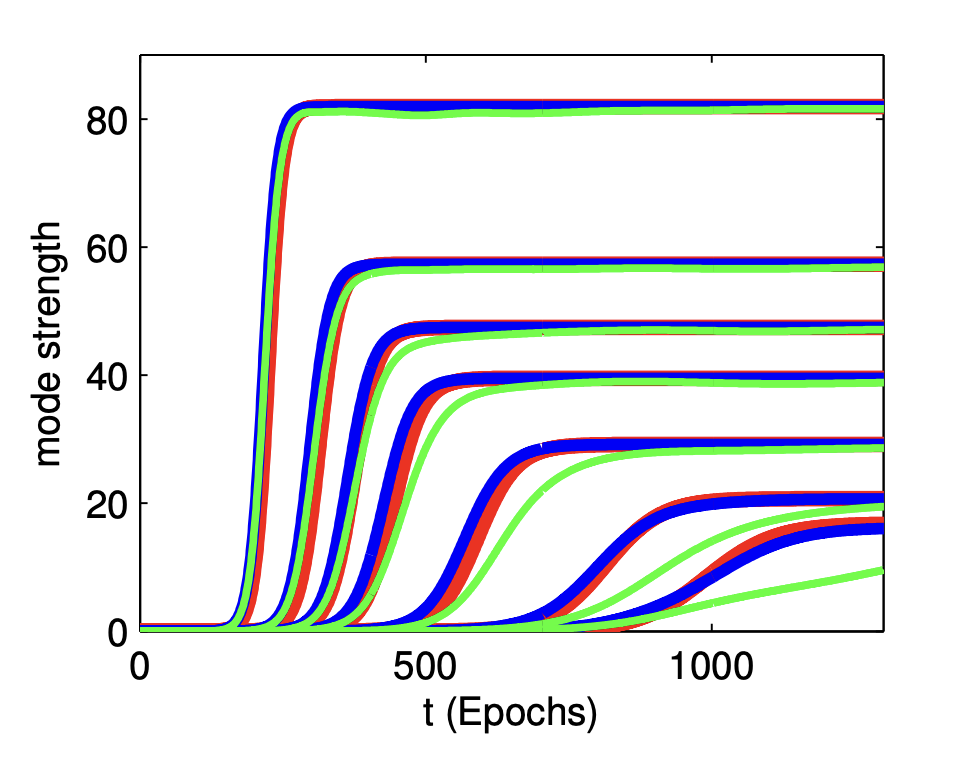
\includegraphics[width=0.4\linewidth]{figures/ch2-svcurves.png}
    \caption{Dynamics of learning in a 2-layer linear network. Curves show the
    strength of the network's representation of seven modes of the input-output
    correlation matrix over the course of learning. Red traces show our analytical
    sigmoids. Blue traces show simulation of the full dynamics of a 2-layer linear
    network from small random initial conditions. Green traces show simulation of
    a \emph{nonlinear} 2-layer network with tanh activation functions.}
    \label{fig:svcurves}
\end{figure}

This illustrates one of the most important tools
in a learning mechanic's toolkit. We rarely get to
prove everything rigorously; the systems are too tangled for that. So instead we
do this: \emph{make a reasonable-looking assumption, derive a theory from it, and
squeeze that theory for concrete, checkable predictions.} Then we go to the
empirics. If the predictions come out tight against reality---as they do here---that
agreement is itself strong evidence, working backward, that the theory is sound
and that the assumption we leaned on was in fact reasonable. A theory that makes sharp predictions and keeps getting them right is a theory
worth trusting.

\section{Saddle-to-saddle training dynamics}

We now have, in the boxed sigmoid from the last section, a complete description of
\emph{how} each mode is learned. The natural next questio is \emph{when}.
If every mode follows its own sigmoid, and each sigmoid switches on at its own
time, then the order and spacing of those switch-on times is the whole story of
the training curve. Let's compute it.

A clean way to summarize ``when is mode $\mu$ learned'' is to ask for its
\textbf{halfway-time} $\tau_\mu$: the moment at which the mode reaches half its
final strength, $s^2_\mu(\tau_\mu) = \tfrac{1}{2}\lambda^\star_\mu$. Setting the
sigmoid equal to $\tfrac12\lambda^\star_\mu$ and solving for $t$ (and dropping
order-one constants, which don't affect the qualitative story) gives a strikingly
simple scaling:\footnote{Filling in this short calculation is left as an exercise
at the end of the chapter.}
\begin{equation}
    \tau_\mu \approx \frac{1}{\lambda^\star_\mu} \ln \frac{\lambda^\star_\mu}{s^2_\mu(0)}.
\end{equation}

Read this formula and a clear prediction jumps out. The learning time is inversely
proportional to the mode strength $\lambda^\star_\mu$: \textbf{big modes are
learned first, small modes last.} And we know from the Canary example what that
means semantically---big modes are the coarse, dominant distinctions in the data
(animal vs.\ plant), small modes the fine subordinate details. So the network
learns the broad strokes of its task before the fine print, and it does so in a
strict, predictable order set entirely by the data's singular values. This is the
precise, quantitative version of the first piece of folklore we opened the chapter
with.

Now look at the \emph{spacing} between consecutive switch-on times, $\tau_\mu$ and
$\tau_{\mu+1}$. Notice the initialization scale $s^2_\mu(0)$ sits inside a
logarithm in the formula: as we shrink the initialization, every $\tau_\mu$ grows,
but they grow by different amounts, and the gaps between them stretch out. The
smaller the initialization, the more cleanly separated in time the modes
become---the sigmoids stop overlapping and instead fire one after another, in
distinct stages.

This is exactly what we see when we plot the loss: a \textbf{staircase loss curve.} Training from small
initialization, the loss doesn't fall smoothly. It sits on a long flat
\emph{plateau}, then drops sharply, then plateaus again, then drops. Our theory tells us precisely what each part of the staircase is: a
plateau is a stretch of time when no mode is transitioning (every sigmoid is
either still off or already saturated), and a sudden drop is the instant a new
mode switches on and the network suddenly captures a new chunk of the data's
structure.

\begin{figure}[H]
    \centering
    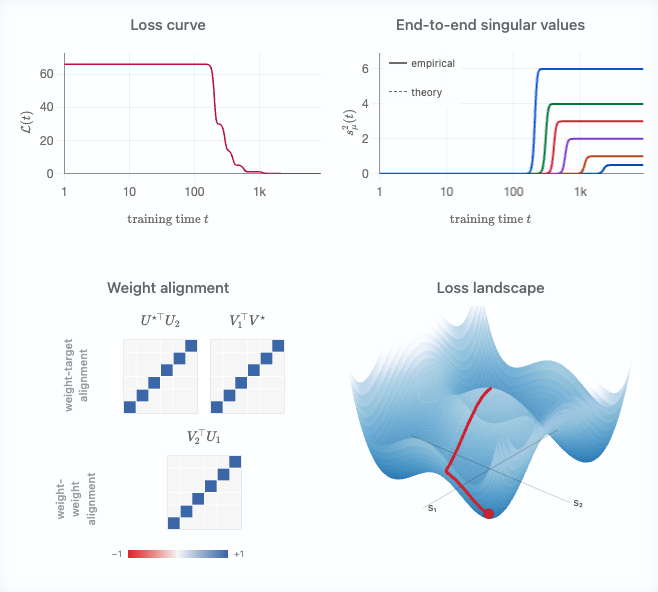
\includegraphics[width=0.65\linewidth]{figures/ch2-saddle.png}
    \caption{As initialization shrinks, the mode sigmoids separate in time and the
    loss curve develops distinct plateaus and drops---the staircase.}
    \label{fig:saddle}
\end{figure}

\subsection{Why the staircase? A landscape full of saddles}

The right way to understand the staircase loss curve is to picture the geometry of the loss landscape.
First we'll show
that the origin---where we start, under small initialization---is a saddle point.
Then we'll see how each mode contributes its own saddle, so that the full
landscape is riddled with them. Finally we'll watch a ball released near the
origin thread its way through this landscape, and the staircase will fall right
out.

\subsubsection*{The origin is a saddle}

Let's zoom all the way in to the simplest possible case---a single mode, with
everything reduced to scalars. The two weights $w_1$ and $w_2$ are just numbers,
the target is a positive number $\lambda^\star$, and the loss is
\begin{align*}
    \Lcal(w_1, w_2) = \tfrac{1}{2}(\lambda^\star - w_1 w_2)^2.
\end{align*}

What does this landscape look like right at the origin, $w_1 = w_2 = 0$? Take the
gradient and you'll find it's exactly zero there: the origin is a flat, stationary
point, a place where the ball, once placed, feels no pull. But ``stationary''
doesn't tell us its shape. Is it the bottom of a bowl (a minimum), the top of a
hill (a maximum), or something else? The way to find out is to stand at the origin
and take a small step in a couple of directions and see which way the ground
tilts.

Step along the direction where $w_1 = w_2$. Their product $w_1 w_2$ becomes
positive, which nudges the prediction $w_1 w_2$ \emph{toward} the target
$\lambda^\star$, so the loss goes \textbf{down}---you're walking downhill.

Now step along the direction where $w_1 = -w_2$. Their product becomes negative,
dragging the prediction \emph{away} from the positive target $\lambda^\star$, so
the loss goes \textbf{up}---you're walking uphill.

A stationary point with a downhill direction \emph{and} an uphill direction is
exactly what we mean by a \textbf{saddle point}; kinda like the surface of a Pringle. The origin is a saddle.

\subsubsection*{One saddle per mode, and a combinatorial explosion of
them}

Now zoom back out to the full, multi-dimensional network. Because the SVD decoupled the dynamics into independent
modes, the total loss is essentially just a \emph{sum} of independent single-mode
losses (this holds in the
aligned, decoupled regime we established in Step 4):
\begin{align*}
    \Lcal \approx \sum_{\mu} \tfrac{1}{2}(\lambda^\star_\mu - s_\mu^2)^2.
\end{align*}

When is the whole network stationary---when do \emph{all} the gradients vanish at
once? Looking at the sum, every mode has to be individually stationary, and we
just learned that each mode is stationary in exactly two situations: either it has
been \emph{perfectly learned} ($s_\mu^2 = \lambda^\star_\mu$, the bottom of that
mode's valley) or it has been \emph{completely ignored} ($s_\mu = 0$, that mode's
saddle at the origin).

Two possibilities per mode, chosen independently, means that if the data has $k$
modes, the landscape has $2^k$ stationary points (within this decoupled mode
picture). That's a lot of places for a ball to get stuck. Let's sort them:
\begin{itemize}
    \item Exactly \textbf{one} is the global minimum---every mode learned,
    $s_\mu^2 = \lambda^\star_\mu$ for all $\mu$. This is the answer we want.
    \item Exactly \textbf{one} is the master saddle at the origin---every mode
    ignored. It's the \emph{highest-loss} of all the critical points (nothing has
    been learned yet), and it's a saddle, because, as we saw in Movement 1,
    stepping away from it along any mode's downhill direction lowers the loss.
    \item \textbf{Every one of the other $2^k - 2$ stationary points is also a
    saddle.} Suppose the largest mode is fully learned
    ($s_1^2 = \lambda^\star_1$) but the second mode is still untouched
    ($s_2 = 0$). Along the first mode's coordinate, the network is sitting
    comfortably at the bottom of a valley. But along the second mode's
    coordinate, it is sitting \emph{exactly on that mode's origin-saddle}, with an
    unexploited downhill direction right there. A point that is a valley-bottom in
    some directions and a saddle in others is, overall, still a saddle. So this
    ``first mode learned, rest ignored'' state is at an
    unstable equilibrium.
\end{itemize}

\subsubsection*{The kinematics of escaping a saddle}

When we initialize with
very small random weights, we are setting the ball down a hair's breadth from the
master saddle at the origin. It starts to roll---but because the weights are tiny,
the gradients are tiny too, and it rolls \emph{excruciatingly} slowly. This is the
source of the very first plateau.

Which way does it go? Recall from Movement 1 that each mode's downhill steepness is
governed by its singular value $\lambda^\star_\mu$---and in fact, near the origin,
each mode's strength grows exponentially at a rate set by $\lambda^\star_\mu$
(this is the power-iteration effect from Step 3). So the ball accelerates down the direction
of the \emph{largest} mode exponentially faster than any other, slides down the
$s_1$ axis, and escapes the master saddle along that one direction.

Then it arrives at the next saddle: $(s_1^2 = \lambda^\star_1,\ s_2 = 0,\ s_3 = 0,
\dots)$---first mode learned, rest still at zero, an unstable equilibrium. Because the gradients for every \emph{remaining}
mode are still microscopically small, the ball slows down and the loss plateaus. But it hasn't stopped. Beneath the surface, $s_2$ is quietly growing,
exponentially, driven by the same power-iteration pull. Eventually it grows large
enough to tip the ball over the edge of \emph{this} saddle, and the ball slides
rapidly down the $s_2$ axis---which we see, up at the level of the loss curve, as a
sudden steep drop. It settles onto the next ledge, and the waiting game begins
again for mode 3. Plateau, drop, plateau, drop. This shows up as a staircase loss curve.

It's remarkable that in this toy example, we're able to make a concrete 
connection between what the network is learning and what the optimization dynamics look like. 
This can be thought of as an instantiation of the learning mechanics idea that learning, at its core,
is movement through high dimensional space.

\subsection{Saddle-to-saddle as implicit regularization}

Notice that because modes are learned in strict order of importance, a
network that we stop \emph{partway} through training will have captured only the
top few modes of $\Sigma_{yx}$, leaving all the rest still pinned near zero. In
other words, gradient descent from small initialization has a built-in preference
for \emph{simple, low-rank solutions}, adding complexity one mode at a time and
only as training proceeds. This is \textbf{implicit regularization} again---the
very phenomenon we met in Chapter 1, where gradient descent on linear regression
quietly preferred the minimum-norm solution without being told to. There, the bias
was toward small norm; here, it's toward low rank. In both cases, gradient descent
is doing something we never explicitly asked it to, biasing itself toward
simplicity.

\section{So what have we learned from all this?}

We started with four pieces of deep learning folklore that seemed like clues to deeper understanding which we wanted to capture in a toy model:
\begin{enumerate}
    \item deep learning learns the components of its target function in a
    preferred order;
    \item deep learning optimizes just fine, despite a wickedly nonconvex loss
    landscape;
    \item instantaneous training dynamics are often low-rank within each weight
    matrix; and
    \item we tend to get stepwise, staircase loss curves, especially when training
    from small initialization.
\end{enumerate}

Deep linear nets capture all of these. So, what now? Did all this reveal any deeper insight into the fundamental reasons for these folklore observations?

By and large, yes! We can revisit each of these four folklore beliefs with a new perspective.

\paragraph{1. The preferred learning order.} We can now say exactly what sets it:
the data, through its covariances. The order depends on the input statistics
($\Sigma_{xx}$) and the target relationship ($\Sigma_{yx}$) together, and the rule
is that larger components of the target along larger directions of the input are
learned faster---precisely our $\tau_\mu \propto 1/\lambda^\star_\mu$ result.
Reassuringly, real \emph{nonlinear} networks share this same bias toward quickly
learning functions of the data's large directions which
is a sign our linear toy model caught something real rather than an artifact of
linearity.

\paragraph{2. Optimizing a nonconvex landscape.} We saw that the fearsome
nonconvex landscape of a deep linear network actually decomposes, after alignment,
into many simple one-dimensional subproblems solved in parallel---one per mode.
This decomposition won't hold exactly for nonlinear networks. But it makes the
folklore far less mysterious, and it dovetails with another widely held belief:
that large models are full of semi-independent ``circuits'' that can be understood
and optimized more or less separately. A landscape that looks hopeless globally
can be benign once you find the right pieces to look at.

\paragraph{3. Low-rank instantaneous dynamics.} In our model, the reason is now
transparent: at any given moment, typically just one singular value (or a few) is
in its rapid-growth phase, while the rest sit still. Each time a singular value
switches on, it opens up a new pathway from input to output---it \emph{looks like
a new circuit suddenly forming.} It’s possible that deep nonlinear networks show low-rank behavior for the similar reason that only a relatively small number of “circuits” are undergoing rapid development at a particular time. Of course, this is highly speculative and this explanation should be handled with care until tested.

\paragraph{4. Staircase loss curves.} This one we explained in full: the
parameters slide down a sequence of saddle points of decreasing order on their way
to a minimum, and the plateaus and drops are the lingering-and-descending of those
saddle-to-saddle dynamics. The same essential mechanism is believed to drive the
staircase curves seen in real nonlinear networks, and deep linear networks are now
the standard, well-understood toy model for the phenomenon.

\bigskip

So the toy model delivered: four behaviors, one solvable system. But let's be
honest about its limits, in the same spirit we were honest about linear regression
at the end of Chapter 1. A deep linear network, no matter how deep, can only ever
represent a \emph{linear} function of its input. Every phenomenon that
fundamentally requires learning a \emph{nonlinear} function of the data lies
completely outside its reach. And that, frustratingly, is \emph{most} of what we
ultimately want to understand about deep learning.

Still---and I hope this is the feeling you're left with---it's remarkable how far
one well-chosen simplification carried us. We kept depth and coupling, gave up the
nonlinearity, and in return got an exact, predictive, empirically validated
account of preferential learning, benign optimization, low-rank dynamics, and
staircase losses. Deep linear networks are the textbook example of a toy model
that is \emph{simple, but not too simple}: simple enough to solve with the tools in
hand, rich enough to teach us something true about the real thing.